\chapter{Introducción específica} % Main chapter title

\label{Chapter2}

En este capítulo se explica en detalle el funcionamiento de un motor de combustión interna. Además, se describe el sistema desarrollado, sus partes y la interacción entre ellas. Y los requerimientos del proyecto.

\section{Funcionamiento de un motor de combustión interna} \label{func-motor}

En la actualidad, el motor de combustión interna es el motor más utilizado en vehículos de transporte de cargas y pasajeros. Existen distintos tipos de motores que utilizan distintos tipos de combustibles. En esta sección se explica, específicamente, el funcionamiento de motores de pistón a gasolina de cuatro tiempos. Estos tipos de motores utilizan un mecanismo llamado cigüeñal para convertir el movimiento lineal que realiza el pistón, en un movimiento rotatorio, que finalmente se transmite a las ruedas del vehículo a través de una transmisión.

En dos revoluciones completas del cigüeñal el pistón pasa por cuatro etapas, representadas en la figura \ref{fig:motor-combustion}
\begin{itemize}
\item{Admisión:} se ingresa a la cámara de combustión una mezcla de aire y combustible, gracias al movimiento hacia abajo del pistón que genera vacío dentro de la cámara.
\item{Compresión:} el pistón se mueve hacia arriba comprimiendo la mezcla de aire y combustible, con esto también aumenta su temperatura.
\item{Combustión:} a través de una chispa generada por una bujía se enciende la mezcla y se produce la combustión.
\item{Escape:} la combustión genera gases que son evacuados de la cámara por el movimiento hacia arriba del pistón. Luego de esta etapa final, el proceso se repite y el pistón vuelve a la etapa de admisión.
\end{itemize}

\subsection{Proceso de combustión y su eficiencia}

Un motor de combustión interna, o motor a explosión, es un tipo de máquina que obtiene energía mecánica a través de una reacción química conocida como combustión. La combustión es la oxidación rápida en presencia de oxígeno de materiales llamados combustibles. El resultado de esta reacción cuando es completa es dióxido de carbono, agua, y energía liberada en forma de calor y expansión gaseosa. La expansión gaseosa es convertida en movimiento rotatorio y el calor se disipa a la atmósfera. Cuando la combustión no es completa, ya sea por exceso o defecto de oxígeno, se producen otros compuestos parcialmente oxidados como el monóxido de Carbono. Esto sucede cuando la cantidad total de energía liberada es menor.

\begin{figure}[htpb]
\centering
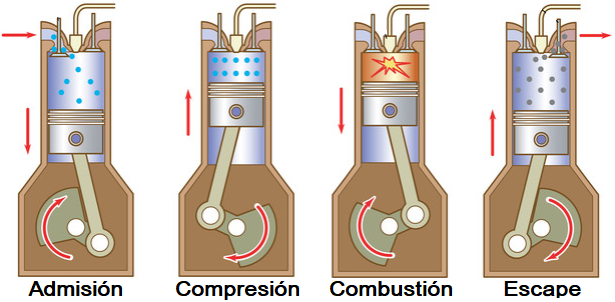
\includegraphics[width=.9\textwidth]{./Figures/motor-combustion.png}
\caption{Representación gráfica de las etapas de un motor de combustión de cuatro tiempos \protect\footnotemark[2].}
\label{fig:motor-combustion}
\end{figure}
\footnotetext[2]{Imagen tomada de \cite{motor}}

Para que una combustión sea completa, se tiene que cumplir la condición de que la proporción por peso, de oxígeno y combustible, sea igual a su proporción estequiométrica. En un motor de gasolina esta proporción es de 14,7 partes de oxígeno por 1 parte de combustible \citep{book-afr}. Se llama factor lambda, denominado con la letra griega $\lambda$, a la relación entre la proporción oxígeno y combustible actual con su proporción estequiométrica. Si la combustión ocurre con exceso de oxígeno, el factor lambda será mayor a 1, si ocurre con defecto de oxígeno, el factor será menor a 1, y si ocurre con la proporción justa será igual a 1. Los sensores desarrollados para poder monitorear este factor son llamados sondas lambda. En los vehículos actuales, el monitoreo de este factor es utilizado para regular la cantidad de combustible inyectada en cada proceso de combustión. De esta forma, es posible operar al motor eficientemente minimizando las emisiones de gases indeseados.

Otra variable que afecta a la cantidad de combustible inyectada es la temperatura de los gases de admisión. La densidad de un gas depende de su temperatura y, como el volumen de la cámara de combustión es fijo, es posible calcular el peso total de oxígeno que puede caber dentro de la cámara. Por lo tanto, es la temperatura del gas de admisión, la que define la cantidad máxima de combustible que puede inyectarse. A menor temperatura del gas, su densidad aumenta y por lo tanto la cantidad de combustible que puede inyectarse, para alcanzar la relación estequiométrica es mayor. Por lo contrario, si la temperatura del gas es alta, la cantidad de combustible que puede inyectarse es menor, y a menor cantidad de combustible, la energía total entregada es menor.

\subsection{Eficiencia mecánica y lubricación}

Solo una parte de la energía mecánica proveniente del proceso de combustión es convertida en energía cinética. Parte de esa energía se pierde por la fricción entre las partes que componen al motor. Para disminuir esta fricción se utilizan fluidos lubricantes, que funcionan impidiendo el contacto entre dos partes móviles. La fricción entre las partes móviles y el lubricante, será menor que la fricción si las partes estuvieran en contacto, y al disminuir la fricción la energía perdida es menor. Para que el lubricante funcione adecuadamente, su viscosidad tiene que estar dentro de un rango definido por el fabricante del motor. Esta es dependiente de la temperatura y por eso es indispensable monitorear o censar esta variable \cite{lubrication}. La temperatura y la viscosidad del lubricante son parámetros proprocionados por el fabricante, y su correcto funcionamiento solo está garantizado dentro de los rangos de valores especificados.

El lubricante es distribuido a las partes móviles del motor a través de un circuito hidráulico cerrado. Este circuito consiste de conductos, un tanque de almacenamiento y una bomba hidráulica. Una presión de aceite insuficiente, puede causar que no sea distribuida a las partes del motor equitativamente, con la posibilidad de causar daños. Por esto, la presión de aceite es monitoreada en forma simultanea con la temperatura.

\subsection{Batería eléctrica}
Los motores no pueden operar sin una fuente de energía eléctrica ya que necesitan de ella para dos procesos importantes: el arranque o puesta en marcha y la ignición del proceso de combustión.
Para arrancar un motor de combustión interna, se utiliza un motor eléctrico que hace girar el cigüeñal y mueve al pistón por sus cuatro etapas. Una vez que se produce la combustión, la propia inercia del sistema hace que la operación sea sostenida. En aplicaciones móviles, el motor eléctrico es alimentado por una batería eléctrica, que por lo general son baterías de plomo y ácido con tensión nominal entre bornes de 12 V. Una tensión baja de la batería puede causar que el motor eléctrico no tenga suficiente torque. Como consecuencia de esto, no podrá hacer girar el cigüeñal, o bien, no alcanzará la velocidad de giro necesaria para encender dicho motor. Por otro lado, si la tensión de la batería disminuye demasiado al intentar arrancar un motor, esto puede indicar que la batería está descargada o que la fricción del motor es muy grande debido a fallas mecánicas o falta de lubricación.

La bujía que produce la chispa necesaria para iniciar la combustión también es alimentada a través de un circuito eléctrico por la batería del motor. Si la batería no tiene tensión suficiente, puede causar que la bujía no genere una chispa o que esta no sea suficiente para lograr la ignición de la mezcla de aire y combustible.

En un vehículo existen otros subsistemas que son alimentados por la batería del motor, tales como las luces, el panel de información, el sistema de audio, etc. Y todos ellos dependen de que la tensión de la batería se encuentre dentro de sus valores nominales para un correcto funcionamiento.

\section{Descripción general del sistema}

El sistema desarrollado consiste de dos partes distintas, la adquisidora de datos y la interfaz gráfica. La primera parte consiste de un circuito controlado por un microcontrolador montado cerca del motor del vehículo. El adquisidor digitaliza las señales producidas por los sensores de temperatura de gases de admisión y escape; temperatura de aceite; sonda lambda; velocidad de giro y tensión de la batería. Los sensores fueron seleccionados según el funcionamiento del motor explicado en la seción \ref{func-motor}.  La información capturada por la parte adquisidora es transmitida a la segunda parte del sistema por \textit{Bluetooth Low-Energy}.

La segunda parte del sistema, la interfaz gráfica, está compuesta por un \textit{Single Board Computer}, una pantalla LCD táctil, y una tarjeta SD para almacenar los datos recibidos. O también puede ser un dispositivo móvil como un \textit{Smartphone} o \textit{Tablet}. La función de esta parte, es mostrar la información recibida en gráficas, e indicar con alarmas visuales y sonoras, cuando el valor de alguna de las variables es superior al límite establecido por el usuario. También, almacena los datos recibidos en la memoria del dispositivo para luego descargar la información y analizarla posteriormente. Esta parte del sistema se encuentra ubicada en la cabina del vehículo en un lugar con fácil acceso y visible para el conductor.

La figura \ref{fig:diagrama-de-bloques} es una representación en diagrama de bloques del sistema.

\begin{figure}[htpb]
\centering
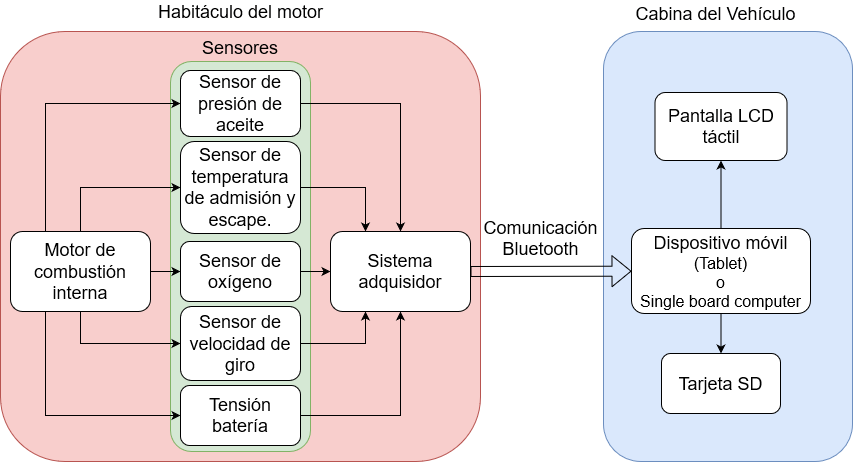
\includegraphics[width=.9\textwidth]{./Figures/diagrama-proyecto.png}
\caption{Diagrama en bloques del sistema.}
\label{fig:diagrama-de-bloques}
\end{figure}

\section{Requerimientos del proyecto}

El desarrollo del proyecto se basó en las historias de usuario y los requerimientos fijados durante la etapa de planificación del proyecto. Los requerimientos se dividieron en cuatro grupos: requerimientos generales del proyecto; requerimientos de la interfaz gráfica; requerimientos de la parte adquisidora de datos y requerimientos de la comunicación entre las partes.

Los requerimientos generales del proyecto son:
\begin{itemize}
\item REQ-GEN-001: todo el código fuente del proyecto será almacenado bajo un sistema de control de versiones GIT.
\item REQ-GEN-002: la documentación del código fuente del software embebido será llevada a cabo en los comentarios, siguiendo el formato de Doxygen.
\item REQ-GEN-003: la documentación del software para la interfaz gráfica también será llevada a cabo en los comentarios. El formato será elegido por el responsable del proyecto.
\end{itemize}

Requerimientos de la interfaz gráfica:
\begin{itemize}
\item REQ-GUI-001: la interfaz gráfica deberá poder mostrar figuras con la información de todos los sensores a la vez.
\item REQ-GUI-002: el usuario podrá elegir qué sensores ver al mismo tiempo y cuáles no desea ver.
\item REQ-GUI-003: el usuario podrá definir alarmas por valor máximo, para cada una de las variables.
\item REQ-GUI-004: las alarmas serán sonoras y visuales. El estilo de las alarmas será definido por el cliente durante el proceso de desarrollo de la interfaz gráfica.
\end{itemize}

Requerimientos de la parte adquisidora:
\begin{itemize}
\item REQ-ADQ-001: el sistema tiene que adquirir la temperatura de los gases de admisión y escape, con un rango de temperatura entre 0 \degree C y 400 \degree C y con una resolución menor igual a 0,5 \degree C. Con una tasa de muestreo mayor o igual a 1 hz.
\item REQ-ADQ-002: el sistema tiene que adquirir la temperatura del aceite del motor, con un rango de temperatura entre 0 \degree C y 400 \degree C y una resolución menor igual a 0,5 \degree C. Con una tasa de muestreo mayor igual a 1 hz.
\item REQ-ADQ-003: el sistema tiene que adquirir la velocidad de giro del motor, en un rango entre 0 y 20.000 revoluciones por minuto, con una resolución menor igual a 500 r.p.m. Con una tasa de muestreo mayor igual a 5 hz.
\item REQ-ADQ-004: el sistema tiene que adquirir la proporción de oxígeno en los gases de escape llamada lambda, con un rango de 0 a 2 y una resolución menor igual a 0,1 lambda.
\item REQ-ADQ-005: el sistema tiene que adquirir la presión de aceite del motor, con un rango de 0 a 100 psi y con una resolución menor igual a 1 psi.
\item REQ-ADQ-006: el sistema debe comenzar a transmitir a la interfaz gráfica la información obtenida en un tiempo no mayor a 1 segundo transcurrido el proceso de adquisición.
\end{itemize}

Requerimientos de la comunicación entre las partes del sistema:
\begin{itemize}
\item REQ-COMM-001: se permitirá que se pierda hasta 1 paquete de cada 100 paquetes transmitidos.
\end{itemize}

\section{Descripción del sistema implementado}

La parte adquisidora del sistema se implementó sobre una placa de desarrollo EDU-CIAA debido a la experiencia de uso acumulada durante el cursado de la Especialización en Sistemas Embebidos. Además, el microcontrolador que utiliza esta placa de desarrollo, el NXP LPC4337, cuenta con los periféricos necesarios para digitalizar las señales de todos los sensores a utilizar y enviar los datos recolectados al módulo de comunicación \textit{Bluetooth}. Específicamente, el microcontrolador posee: interfaz SPI de cuatro canales con velocidad hasta 60MB por segundo; interfaz USART, y tres conversores analógico digital de 10 bits de resolución y tasa de muestreo de 400 mil muestras por segundo.

Para la comunicación \textit{Bluetooth} entre las partes se utilizó el módulo HM-10, basado en el circuito integrado CC2541 de Texas Instruments. Se utilizó este módulo porque sus niveles de señales son compatibles con los de la EDU-CIAA, tiene un bajo consumo de energía y puede transmitir información serie con una velocidad de hasta 6 kilobytes por segundo \cite{HM-10}.

Para la interfaz gráfica se utilizó una \textit{Raspberry Pi 3B+} con una pantalla LCD táctil capacitiva de 5 pulgadas de longitud diagonal y resolución de 800 píxeles de ancho por 480 píxeles de alto. Se eligió esta plataforma porque posee comunicación \textit{Bluetooth Low-Energy}, utiliza un sistema operativo basado en Linux y puede correr scripts escritos en Python 3.7 \cite{raspberrypi}.

Para cumplir con el requisito REQ-GEN-001, se utilizó \textit{Git} para el control de versión para los proyectos del circuito impreso y el software desarrollado. Se mantuvieron copias almacenadas en el servicio gratuito proveído por \textit{Github.com}. 

\section{Sensores y selección de hardware}

\subsection{Sensor de temperatura}

Para medir las temperaturas de los gases de admisión, escape y temperatura de aceite se utilizaron termocuplas tipo K. Una termocupla es un dispositivo compuesto por dos alambres metálicos de distintos materiales unidos en un punto. Cuando existe una diferencia de temperatura entre la unión y su extremo abierto, se genera una diferencia de tensión en sus bornes. La tensión generada es proporcional a la diferencia de temperatura, a este efecto se llama efecto Seebeck \cite{termocupla}. Para convertir la tensión de la termocupla en un valor de temperatura, se utilizó el circuito integrado MAX31855K.

\subsection{Sensor de presión de aceite}

El sensor de presión de aceite es un sensor de resistencia variable. Su valor de resistencia entre bornes es proporcional a la presión sensada. El sensor utilizado tiene un rango de 0 a 120 psi y su valor de resistencia va de 7 a 132 Ohm.

\subsection{Sensor de factor lambda}

Una sonda lambda, es un sensor que produce una señal eléctrica de tensión proporcional al factor de oxígeno sensado. El sensor utilizado puede medir factores lambda entre 0,8 y 2. Para la medición de esta variable fue necesario utilizar un circuito integrado especializado. El LM9044, fabricado por Texas Instruments, es un amplificador diferencial diseñado para leer la señal de una sonda lambda con un conversor analógico digital.

\subsection{Sensor de reluctancia variable}

Para medir la velocidad de giro del cigüeñal del motor se utilizó un sensor de reluctancia variable. Estos sensores convierten variaciones en la reluctancia magnética en una señal de tensión. Estas variaciones, son generadas por la presencia o movimiento de un objeto ferroso en la proximidad del sensor. La medición de la velocidad de giro del cigüeñal se hace a través de una rueda fónica. Una rueda fónica es una rueda dentada de acero que gira en conjunto con el cigüeñal del motor. Cuando la rueda gira, los dientes se acercan y se alejan del sensor y esto genera un tren de pulsos en sus bornes. Para medir la velocidad de giro, la señal del sensor tiene que ser convertida a una señal cuadrada de valores de tensión dentro del rango admisible por el microcontrolador. Para esto se utilizó el circuito integrado MAX9924 \cite{MAX9924}. El proceso de adaptación de la señal del MAX9924 está representado en el diagrama de bloques de la figura \ref{fig:bloq-rpm}.

\begin{figure}[htpb]
\centering
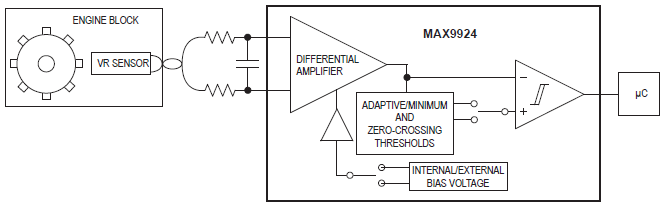
\includegraphics[width=.9\textwidth]{./Figures/max9924.png}
\caption{Funcionamiento del MAX9924 representado en diagrama de bloques. \protect\footnotemark[4].}
\label{fig:bloq-rpm}
\end{figure}
\footnotetext[4]{Imagen tomada de \cite{MAX9924}}